\documentclass{article}
\usepackage[margin=1in]{geometry}
\usepackage{graphicx}
\usepackage{amsmath}
\usepackage{multirow}
\usepackage{multicol}
\usepackage{wrapfig}
\usepackage{algpseudocode}



%\topmargin 0pt
%\oddsidemargin 12pt
%\evensidemargin 12pt
\interfootnotelinepenalty=10000


\begin{document}
\title{Unsupervised Learning Segmentation of Objects in a Scene\\
\large  Project in COMP 652 and COMP 765}
\author{Yi Tian Xu\\260520039}

\maketitle

\abstract{Unsupervised learning segmentation is beneficial for autonomous robots to reason and manipulate objects in their environment when supervised data becomes both expensive and insufficient. We employed the idea of using action to delimiter segments, and developed a filtering method to extract foreground and a probabilistic matching method to track and infer object segments. We conducted experiments in a scene with rigid objects and concluded that the construction we have so far requires more tuning and optimizations to be considered as a viable solution.}

%\begin{multicols}{2}

\section{Introduction}
Object manipulation and cognition are arguably a highly coupled task. For example, human infants can develop their manipulation skills through imitation \cite{cogn1}. For an autonomous robot, we thus image it to be driven by a continuous sequence of action, perception and reaction. In particular, it needs to identify and reason about its surrounding objects that potentially lies in a dynamic and unstructured environment. 

Recent studies in neural networks, in particular, Fully Convolutional Network (FCN) \cite{fcn} and Mask RNN \cite{rnn}, have risen as powerful tools in segmentation. Yet, as any supervised methods, a pre-defined labelled dataset provided by a human teacher may limit a robot in its reasoning about novel objects. Moreover, robots who work in a specialized field (e.g.: pruning of city trees) may have supervised data that can be expensive to obtain, while robots with multi-dimensional specialities (e.g.: a eldercare home robot) may require an extensive amount of data to cover all cases exhaustively.

In this work, we address to the problem of objects segmentation based on an unsupervised approach. We use motions to determine object boundaries and a probabilistic matching method to infer and track the segments. In our setting, we will consider a passive robot that observes objects moved by a hand in its environment.

\section{Related Works}

Past studies have attempted to used robot's actions to coordinates its reasoning in detecting segments. For example, Hoof et al. \cite{herke} partitioned the environment into parts tracked by local key point descriptors, and developed a probabilistic model to infer the labelling of each part and to select best action to maximize information gain. As their approach rely on visual features detectable through Scale Invariant Feature Transform algorithm, the robustness to textureless objects is weak. Another disadvantage is that they ignore continuous observation of the objects and hand motion. Instead, they took snapshots of the scene before and after the robot's action, and use Random Sample Consensus algorithm to find a rigid 3D transformation to track the parts. Due to a 1\% inaccuracy in their tracking algorithm caused by, for example, illumination change and occlusion, the tracking error was accumulated through time, and prevented the robot to correctly infer the number of segments in their experiment. 

Hoof et al. mentioned that their method is independent of the type of descriptor employed provided that the set of key points is sparse and each can be detected reliably from multiple views. Thus, expanding their method to low-texture object may simply require adding a new type of descriptors. However, we suggest that the use of continuous motion observation can provide enough information to track the parts without tracking key points. The main concern remains to segment the hand from the moved object.

Correlation between the hand movement and the moved object may impose a challenge in discriminating the robot hand from touched object. Fitzpatrick et al. \cite{max-flow} experimented on segmenting one object of interest by making an impact movement on that object. They suggested to isolate the motion of the hand from the motion of the targeted object by comparing the result from the image differencing before and after the moment of impact. We adopt their idea of using image differencing and attempt to expand their method to general hand-object movements and co-movement of objects.

\subsection{Tracing Object Boundaries}

As image differencing relies on the difference between pixel values in consecutive frames, it allows us to obtain a thin object boundary depending on the direction and the speed of the motion. Fitzpatrick et al. \cite{max-flow} used a maximum-flow algorithm for vision \cite{kolmo} to find the interior region of the object boundary. As am attempt for improvement, we will try to obtain a thicker object boundary allowing us to quickly fill the interior of the object. 

Intuitively, if we trust that millions years of evolution has already provided us the optimized example of a vision system in ourself, would a biologically more plausible solution exceeds the performance of the maximum-flow algorithm in vision? A popular method for edge detection in computer vision inspired by the visual cortex consists of convolving different oriented Gabors with the image and pulling the maximum value: Gabor filtering. Gabors also have reputation in image classification and object recognition tasks with convolutional neuro networks (CNN). Gabor filters are often found at the top layers. In conjunction with the biological findings, the use of Gabor filters in a CNN is by some called a \emph{standard model}. \cite{Gabor}

In our method, we will employ Gabor filtering to detect the edges and use Gaussian blurring to thicken and smooth them. 

\subsection{Image Region Tracking and Matching}

Object tracking based on points or descriptors, as in the work of Hoof et al. \cite{herke}, holds several challenges. Also discussed in the survey by Yilmaz et al. \cite{tracking}, such tracking requires some measurement of correspondence based on the motion of the tracked points or the entire object. Furthermore, the set of tacked key points often varies from frame to frame; old key points may become occluded and new key points may appear. Thus, as Hoof et al. argued, a probabilistic approach represents a suitable solution to handle missing data and noisy observations.

In the context of multiple objects segmentation, reasoning in the movement correlation between tracked image regions may rise a concern in the trade-off between the number of regions tracked and the computational complexity. In Hoof et al.'s probabilistic method \cite{herke}, for example, tracked key points are initially partitioned into parts by a 3D grid covering the observed environment. Each part connects to a hidden markov model with known action and observed motion state, and latent segmentation labelling and true motion state. The computation of the probabilities growns exponentially as the number of parts increases. They therefore resort to Gibbs sampling to approximate the distribution. 

Shape matching represents an alternative approach to key points tracking \cite{tracking}. Shape, usually detected by background subtraction, can be complete object regions and large enough to overlap between frames. Matching is can be based on a similarity score with the hypothesized object segment generated by the previous frame. For example, Park et al. in their work for tracking and segmenting interacting human body parts \cite{human-action} employed many criteria to reason about image region similarity, namely color, border, size, orientation, neighbouring regions, etc. Others, mentioned by Yilmaz et al. \cite{tracking}, modelled shapes by color and edge histograms and used Bhattacharya distance or Kullback-Leibler divergence to establish similarity. Histogram is invariant to translation and rotation, and normalized histogram is invariant to scaling, providing convenience for representing shapes and evaluating similarities.

A motion-based approach to shape matching discussed by Yilmaz et al. \cite{tracking} is to evaluate the optical flow within the shape and use the dominant velocity vector to point to the corresponding shape in the next frame. This approach relies less on appearance invariance, which can be a solution to come of the crucial challenges in Park et al.'s image region matching problem.

Park et al. \cite{human-action} raise the concern that a single shape can split to multiple shapes on the next frame and, similarity, multiple shape can merge into one. In contrast to key points matching, shape matching is many-to-many and they can also appear and disappear from one frame to another. While Park et al. resolved their matching problem using multiple bipartite graph matching combined with hand turned heuristics, we attempt to use a combination of color-histogram-based and optical-flow-based approach to track image regions and to match them to previously inferred segments. 

\subsection{Image Mutual Information}

Aside its application in tracking, mutual Information (MI) has been a common measurement tool for image comparison in clinical applications \cite{mi}, in particular for aligning 2D images to form 3D images. At the heart of the technique is the designation of the marginal and joint histogram as the image distribution. In this formulation, each pixel is a random variable. The marginal histogram counts the occurrence of pixel values in the image, which is 1-dimensional, while the joint histogram counts the co-occurrence of pixel pair values in two image, which is 2-dimensional. 

Marginal and joint histograms are then used to compute marginal and joint entropy, which are finally used to compute MI. Maximizing MI over images transformation (e.g.: rotations and translations) approximates the best alignment. This assumes a statistical relationship between two images which can be captured by the joint entropy. Maximizing MI is thus related to minimizing the joint entropy. Yet, the joint entropy may encounter problems when used alone, as argued by Pluim et al. \cite{mi}. For example, when one image is wildly transformed from another, some regions in the background may produce a peak in the joint histogram, reducing the joint entropy. In the context of shape matching, simply matching to a smaller shape can reduce the joint entropy.

The independence of visual features and the lack of parameter tuning have given MI success in the medical domain. Pluim et al. \cite{mi} showed in their survey a diversity of variation of MI, including normalized MI and MI that includes spacial information by consider one neighbouring pixel value. Russakoff et al. \cite{rmi} proposed regional mutual information, extending the idea of spacial information inclusion by considering all neighbouring pixel in a $nxn$ neighbourhood, creating $n\times n$-dimensional marginal histograms and $2n\times n$-dimensional joint histograms. Computational complexity can be optimized using PCA and the performance is asymptotically close to the original MI as the neighbourhood radius is fixed. 

Although Russakoff et al. showed that RMI is more robust to noise than the original formulation of MI and the variations explored by Pluim et al, we will use the original formulation of MI as a measure to match segments between frames and to experiment its performance in our problem context. 

\section{Method}

\begin{figure}[tbp]
\begin{center}
\caption{Visualization of the method: (A) Input frame is being processed to (B, C, D and E). (B) Background average is accumulated with the new frame. (c) Image difference detects movement. (D) Gabor filtering detects edges in the current frame (also on the background (B), not shown in image). (E) Image differencing between Gabor filtered background and (D) results image parts that can be mapped to segments. (F) Finally, a probabilistic matching method infers and tracks the labellings of the parts in (E) according to the previously inferred segments and the observed motion in (C).}
  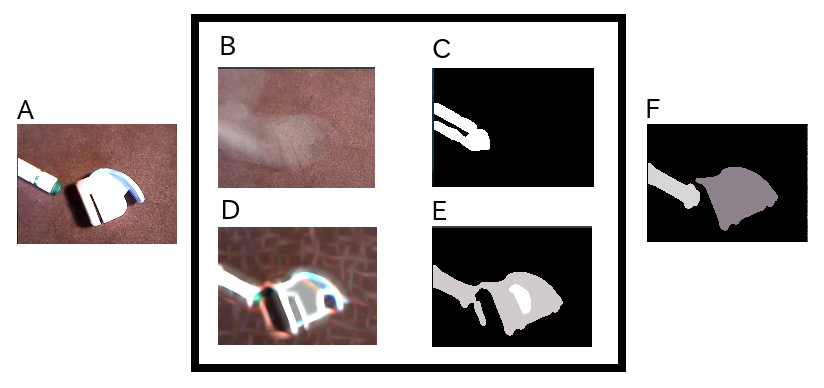
\includegraphics[width=0.9\textwidth]{1}
\label{figure:model_seq}
\end{center}
\end{figure}

Our method is composed of two stages. The first stage segments the moved objects (or the foreground) from the background. The second stage uses the retrieved information from the first stage to infer and track the segments. Figure \ref{figure:model_seq} illustrates the method.

\subsection{Filtering and Part Extraction}

At each frame, we add the frame to the background average and we use image differencing to detect motion. We compute the area of each contour in the resulting image to decide whether a considerably large motion has occur. This prevents detecting false-positive motion due to noise caused by shadows or change in illumination. If at least one contour has a large enough area, we preform Gabor filtering on the background average and the most recent frame. In our experiment, we used $n_g=$ 4 differently oriented Gabors of $s_g=$ 12 px in size. A second image differencing between the two filtered images, which is equivalent to a background subtraction, yields isolation of moved edges. 

To obtain a clean image of the moved edges, we need to add a few other filters before and after the Gabor filters, namely Gaussian blur and thresholding. Below is the pseudocode for parts extraction.\\

\begin{algorithmic}[H]
	\Function{PartsExtraction}{RGB image frame $I$, RGB background average $B$}
		\State $I' \leftarrow$ GaborFilter($I$)
		\State $B' \leftarrow$ GaborFilter($B$)
		\State $P \leftarrow$ AbsoluteDifference($I'$, $B'$)
		\State $P \leftarrow$ GaussianBlur($P$, $\sigma$)
		\State $P \leftarrow$ Thresholding($P$, $\theta_1$)
		\State $P \leftarrow$ SplitIntoContours($P$, MIN\_COUNTOUR)
		\State \Return $P$
	\EndFunction 
\end{algorithmic}

\begin{algorithmic}[H]
	\Function{GaborFilter}{Image $I$}
		\State $I_1 \leftarrow$ GaussianBlur($I$, $\sigma$)
		\State $I_2 \leftarrow I_1$
		\For{each Gabor kernel $k$}
			\State $I_2 \leftarrow \max$(Convolution($I_1$, $k$), $I_2$)
		\EndFor
		\State $I_2 \leftarrow$ Thresholding($I_2$, $\theta_2$)
		\State \Return $I_2$
	\EndFunction
	
\end{algorithmic}

The Gaussian blur preforms a Gaussian averaging for each pixel with a neighbouring spread of $\sigma$. The thresholding segments the image into two parts with the cutoff pixel value $\theta_i$. The parameter $\sigma$ is tuned to 11 in the experiment. 

The size of the Gaussian blur ($\sigma$) affects the performance of the Gabor filters. We added blurring prior to the Gabor filter to soften the shadow and to smooth the extracted edges (see Figure \ref{figure:gaussian_blur}). A additional Gaussian blur is used after the Gabor filter accompanied with thresholding to smooth further the edges and to remove noise. 

\begin{figure}[tbp]
\begin{center}
\caption{Comparison between non-blurring (B, C) and blurring (D, E) prior to Gabor filtering. (A) The original scene frame.  (D) Detected edges without Gaussian blur prior to Gabor filtering, and (C) with Gaussian blur and thresholding after Gabor filtering. (D) Detected edges with Gaussian blur prior to Gabor filtering, and (E) finalized with another Gaussian blur and thresholding.}
  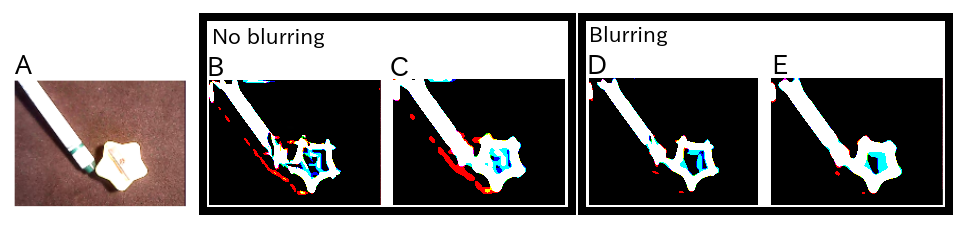
\includegraphics[width=0.95\textwidth]{2}
\label{figure:gaussian_blur}
\end{center}
\end{figure}

The last operation in the parts extraction function, \emph{SplitIntoContours}, finds the contours and fill-in colors. This is a quick heuristic to segment moved object from the background, assuming that all objects have no hole that reveals the background inside them (e.g.: a doughnut-shaped object). The obtained segmentation is used as partitioning of the image that shall be fed to the probabilistic matching method to infer and track object segments. 

\subsection{Probabilistic Matching}

Scoring similarity may not necessitate a probabilistic approach as simply maximizing a similarity scores can be enough to find the best matching. However, since the set of elements to match changes from frame to frame, modelling each inferred segment as a normalized weight vector of labellings may be more intuitive in three ways: (1) ambiguous image regions can be resolved after observing more evidence(s) (2) uncertainly in the appearance or disappearance of a segment can also be capture in the probabilistic model, and (3) normalization enables comparison of scores between different inferred segments. 

\subsubsection{Similarity Measure}

Both the motion detected through image differencing (which we will call \emph{motion image} henceforth) and the image with the extracted parts are considered in our probabilistic matching model. Let $R_t$ be a part extracted at time $t$ and $M_t$, the motion image computed at the same time. We compute the probability of $R_t$ being labelled by $l$ given motion image as
\begin{equation}
	P(R_t = l | M_t) = \sum_{S_{t-1}} P(R_t = S_{t-1} | S_{t-1}, M_t)P(S_{t-1} = l)
\end{equation}
where $S_{t-1}$ is the segments inferred from the previous time step. $P(R_t = S_{t-1} | S_{t-1}, M_t)$ is estimated using MI between the newly extracted part, the previous inferred segment and the motion image. We assume that 
\begin{equation}\label{eq:blab}
	P(R_t = S_{t-1} | S_{t-1}, M_t) \propto F_{MI}(R_t; S_{t-1})D(F_{MI}(R_t; M_t) + \epsilon, F_{MI}(S_{t-1}; M_t) + \epsilon)
\end{equation}
where
\begin{equation}
	F_{MI}(A;B) = \frac{MI(A;B)}{H(A)}
\end{equation}
where $MI$ is the image mutual information and $H$ is the entropy function. We found that $F_{MI}$ is a more suitable score to establish similarity in this context. As MI is not upper bounded, reasoning in whether a MI score is large enough to determine a matching as opposed to no matching at all is not well-defined. Different from the medical application where a true image alignment is usually guaranteed to exists, our context often encounters the case when the extracted part $R_t$ is truly a new segment. In such case, maximizing MI between previously inferred segments will inevitably give the wrong solution. We therefore normalize MI with the extracted part's entropy to upper bound the score by 1. The score is exactly 1 when the compared images are identical. 

Equation \ref{eq:blab} thus conducts three comparisons. The similarities between $R_t$ and $M_t$, and $S_{t-1}$ and $M_t$ are combined and reweighed by the function $D$. Intuitively, image parts and inferred segments are probabilistically more likely to match if they are both matching the motion image, or both not matching the motion image. In other words, the matching should be consistent with the observed motion. Thus, we choose
\begin{equation}
	D(A,B) = -\log\left(1-\min\left(\frac{A}{B}, \frac{B}{A}\right)\right)
\end{equation}
The choice of using the minimum ratio between $A$ and $B$ is to bound the range of $D$ between $0$ and $\infty$. The negative logarithm function will allow $D$ to increase rapidly as $A$ and $B$ becomes closer in value. Since the function is undefined when $A$ or $B$ equals to 0, we add a small value, $\epsilon$, in Equation \ref{eq:blab} to ensure that the input is never 0. In the context of Equation \ref{eq:blab}, $D$ will reach maximum value only if comparisons of the regions $R_t$ and $S_{t-1}$ with the motion $M_t$ yield identical $F_{MI}$ values. $D$ will tend to 0 when the $F_{MI}$ values are largely different. As $F_{MI}$ is designed to measure image similarity, $D$ is designed to measure similarity of similarity values. 

Other function choices for $D$ can also be considered. For example, we can also choose to have $D$ increase linearly or in a polynomial fashion. The percentage difference, the Euclidean distance, standard deviation, etc, can also shape the design for $D$. However, in experiment, the rapidly growing $D$ appears to be more suitable to our method. The other options were often, if not always, unable to segment a moved object from a still object after both object were tagged with the same label.

In our implementation, we further upper-bound $D$ by a large value to avoid numerical issues and to enable normalization of the scores. 

Note that when we compare the images, we use the extracted parts, the inferred segments and the motion images as masks. Histograms are computed using the original frames applied with the mask; the current frame is used for $R_t$ and $M_t$ and the previous frame is used for $S_{t-1}$. At the end of each iteration, extracted part $R_t$ will update a previously inferred segments $S_{t-1}$ by replacing its mask and labelling probabilities if $\mbox{argmax}_l P(R_t = l|M_t) = \mbox{argmax}_l P(S_{t-1} = l)$.

\subsubsection{Appeared and Disappeared Image Regions}

Park et al. mentioned that object segments can appear and disappear due to occlusion, shadowing and overlap \cite{human-action}. To address to this issue, we introduce a segment decay parameter $\alpha$, which we set to 0.05 in our experiment. At each time step, each inferred segment will have all their label probability reduced by $\alpha$ (i.e.: $P(S_{t} = l)$ for every segment $S_t$ and labelling $l$ is updated to $(1-\alpha)P(S_{t} = l)$ at the end of each iteration). If the segment is no longer matched to any newly observed image part(s), it will keep decaying. 

The decay factor applied onto the labelling probabilities after $\tau$ consecutive times steps with no matching is $(1-\alpha)^{\tau}$, implying a probability of $1- (1-\alpha)^{\tau}$ that the decaying segment should be assigned to a new labelling. It would be inappropriate to use this implication directly to decide whether a new labelling should appear because old segments should not suddenly change their labelling. Instead, we called this probability the "decay weight" of corresponding segment ($d_{S_t}$) and use the average of the decay weights over all inferred segments rescaled by the variance of the comparison scores of an extracted part to decide whether that part should be assigned to a new labelling. 

The reason for using the variance (or standard deviation) in the decision of adding new labelling refers to the idea that an image part that is equally similar to all previously inferred segments should either matches all those segments or none of them depending on how similar it is to all those segments. As explained in the previous section, it is for this reason that an upper bounded similarity score becomes crucial in this matching problem, and our $F_{MI}$ function can provide the need. 

In summary, the probability for part $R_t$ to be aligned to a new label $l'$ is 
\begin{equation}
	P(R_t = l' | M_t) \propto \frac{1}{n_{t-1}\mathcal{S}(R_t, M_t, C)} \sum_{S_{t-1}}(d_{S_{t-1}})
\end{equation}
where $n_{t-1}$ is the number of inferred segment at time step $t-1$ and $\mathcal{S}(R_t, M_t, C)$ is the standard deviation of the similarities scores as computed by Equation \ref{eq:blab} over all inferred labelling scaled by some constant $C$. In our experiment, we choose to multiply the standard deviation by $c = 100$. In the case when there is only one inferred segment, we set $\mathcal{S}(R_t, M_t, C) = 1$. 

At the end of iteration, we can filter out segment with a large decay weight.

\subsubsection{Merging and Splitting Image Regions}\label{sec:splitting}

Park et al. also mentioned that previously inferred segments can split or merge into others also due to similar optic effects \cite{human-action}. For our method, we analysed in detail the possibilities of merging and splitting to further decide whether more software architecture is needed handle each case. Through our experiment, we observed four main causes:
\begin{itemize}
	\item Noise caused by shading, shadowing and change in illumination can cause false segmentation or a segment to split into various parts. 
	\item Co-movement of objects and objects touching or overlapping each other can result one part extracted for two or more segments.
	\item An previously moved object will stay visible for some time in the background subtracted image; its exit is a gradual fade, which may cause shrinkage and splitting of the object boundary detected in the part extraction algorithm. 
	\item Background subtraction is itself imperfect at foreground segmentation when movement happens after foreground has stopped moving long enough to be averaged into the background.
\end{itemize}

We notice that all four causes are due to the part extraction algorithm which rely on accurate and precise segmentation between moved object and still objects. Moreover, background subtraction induce another type of segment degeneracy: segment shrinkage. One solution to avoid segment shrinkage is to not match parts that did not moved to any previously inferred segment. However, the mask created with our motion image, which is the only information we have that exclusively captures the motion between two consecutive frames, may cover regions belonging to still objects due to overlap and noise. Thus, reasoning which extracted parts are still objects is not trivial. 

The ideal option may be to replace background subtraction or the entire part extraction algorithm with a solution that not only can segment the hand from the co-moving object, but also produce accurate and precise foreground segmentation. Such option can be left for future investigations. Therefore, we decided to only handle the first two causes for segment merging and splitting.

Note that occluded objects that are previously segmented will have no match on the frame where they are occluded. Thus, if a object was previously segmented, it can still stay segmented when occluded for some time under the condition that we correctly handle the transition between visible, to overlapped and finally to occluded. Similarity, the inverse transition can also happen. Thus, we hypothesize that our method can handle occlusion to some extend if it can handle overlap.

Noises result random appearance of small parts which can be simply filtered out by conditioning on the size of the extracted part. Merging and splitting inferred segment can simply done by replacing multiple inferred segments with the most likely matched part and one inferred segment with multiple most likely matched parts respectively. Nonetheless, the main complexity in this matching problem lies in the merging and splitting of extracted parts. 

Merging requires merging of the labelling probabilities, which at worst, can be recomputed with the merged part. Yet, what to do if the most likely labelling of the merged part differs from the one from the individual parts? Or perhaps, it is better to not merge image part at all. Yet, since the number of comparisons grows exponentially in the number of elements to compare, part merging presents a benefit for the computational complexity.

Let $\pi_{P_i}$ be the vector of probabilities for part $P_i$. Suppose that label $l$ has maximum probability for all $P_i$ for $i\in \{1,...,k\}$, i.e.: $\max_j \pi_{P_i}[j] = \pi_{P_i}[l],  \forall i\in \{1,...,k\}$. After merging, we recompute the probability of the merged part for each labelling, obtaining merged part $P'$ and probability vector $\pi_P$. We can further compare $\pi_P[l]$ with the $\pi_{P_i}[l]$, perhaps by assessing whether $\pi_P[l] > E[\pi_{P_i}[l]]$ or $\pi_P[l] > \max_i (\pi_{P_i}[l])$. This may serve as a measure for deciding whether to keep the merging or not. However, we decided to not conduct any of such evaluation and simply merge the parts without regret.

On the other hand, to decide whether a part should be slitted, we find the inferred segments that are most likely to be matched to the part. If the part also has high probability to be matched with the segments, we split it. 

Splitting required the knowledge of exact positions to split. The matching inferred segments may be informative to suggest those positions, yet we are unclear in how exactly those segments can help in deciding where to split. Therefore, we instead employ the motion-based shape tracking approach that computes the optical flow between the previous frame masked by the inferred segments and the current frame masked by the part. We use the average flow vector to update the position of the segment, and the part with its labelling probabilities are discarded. 

\section{Results and Discussion}\label{sec:exp}

We used OpenCL software package and ROS to implement our method for a "single-eye robot". The camera is stationary in a scene with initially zero to three objects. Objects are moved by a hand (either a human hand or a stick) and are free to leave the camera's field of view. To allow our method to run close to real-time, we had to downside the frames to 160 $\times$ 120 px, which allowed the matching algorithm to run around 3 Hz. 

\subsection{Segmentation}

Various parameter tuning were conducted for the part extraction algorithm. In particular, the sizes of the Gabors filter and the Gaussian blur, and the two thresholds $\theta_1$ and $\theta_2$ were manually tuned together. We observed that, for an image size of 160$\times$120 px, Gabors of size 14 and 16 px were often resulting noisy edges that were touching between objects. A size equal or larger than 18 px, or smaller than 12 px were lacking in responsiveness to the edges, thus resulting often missing parts. We therefore use size of 12 px for the Gabors.

We also observed that a mean ($m$) pixel value around 95 (maximum is 255) and a standard deviation ($s$) around 40 after Gabor filtering gives our best result so far for foreground segmentation. $\theta_1$ needs to be high enough to only filter in edges and $\theta_2$ need to be low enough to dilate the edges. We found that $\theta_1 = \min(\max(150, 1.7s+m), 200)$ and $\theta_2 = s$ appears to give the best result so far. Automatic turning of these parameters and metrics for evaluating the goodness of a segment for our method can be subjected to future research.

Our choice of using Gabor filtering with background extraction fulfills the need of distinguishing the hand from the moved objects. As shown in Figure \ref{figure:many}, objects that were preciously moved stay detectable in the part extraction algorithm after the hand moves away from the objects. 

For segmenting complex object, e.g.: a human hand, we observed that the shading may hinder the object boundary detection done with the Gabor filters. As shown in Figure \ref{figure:hand}, the shaded area of the hand has low contrast with the background, resulting an incomplete detected boundary. Human hand, as we observed, often has multiple parts that are never merged into one segment. The parts usually appears one after another as the hand takes some times to enters the scene. Since we do not consider motion correlation between already inferred segments, no rules is made for reasoning about segments that are often, if not always, observed to move together. Unless one part can be extracted to match both segments, these segments will never be merged. 

Our current part extraction algorithm lacks robustness in finding the complete and precise object contour. It is also biased to object that is lighter in color compared to the background (see Figure \ref{figure:int}). We explained this effect by the Gabors elevating the contrast at the edges by increasing intensity of lighter regions and decreasing that of darker regions. Therefore background subtraction will detect the region around the darker objects, but the region within lighter objects. Perhaps one can extend the method by integrating the intensity inverted image. Future improvement of the algorithm can be beneficial for the method's generalizability.

\begin{figure}[tbp]
\begin{center}
\caption{Moving with human hand. From left to right, the frame, the Gabor filtered frame and the extracted parts. We see that the hand is split into two parts. The leftmost hand's part appears before the rightmost part as the hand sweeps into the scene from right to left.}
  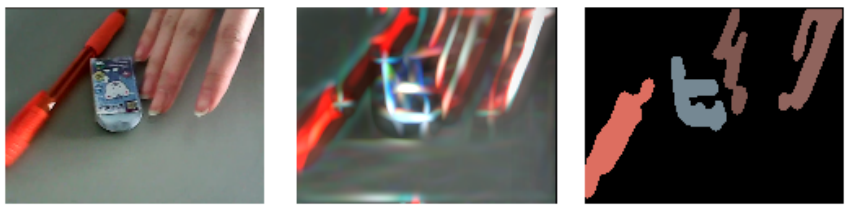
\includegraphics[width=0.65\textwidth]{5}
\label{figure:hand}
\end{center}
\end{figure}

\begin{figure}[tbp]
\begin{center}
\caption{Moving many objects in a scene. From left to right, the frame, the background average, the Gabor filtered frame and the extracted parts. An orange pen was used to move the objects.}
  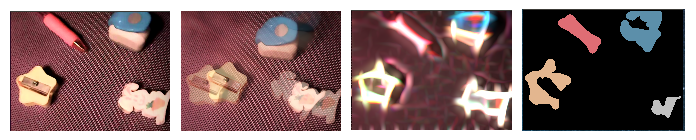
\includegraphics[width=0.75\textwidth]{6}
\label{figure:many}
\end{center}
\end{figure}

\begin{figure}[tbp]
\begin{center}
\caption{Comparison of the foreground object intensity relative to the background. From left to right, the frame, the Gabor filtered frame, the extracted parts and the masked frame with the extracted parts. The two pens, one in back and one in orange, are placed on a brown textured background. The part extracted for the darker pen is are contour of the pen.}
  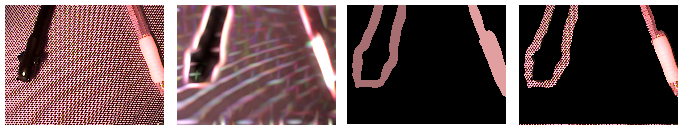
\includegraphics[width=0.75\textwidth]{4}
\label{figure:int}
\end{center}
\end{figure}

\subsection{Inference and Tracking}

As our part extraction was lacking generalizability to dark objects (relative to the background) and complex shaped objects (e.g.: human hand), we preform a set of experiments on dark-colored backgrounds for testing tracking, splitting and merging. Some relevant results are shown in Figure \ref{figure:res}. 

\begin{figure}[tbp]
\begin{center}
\caption{Relevant results. Examples are ordered from top to bottom. From left to right, we name the image types: row (A), the frame, the background average, the motion image and the inferred segments; row (B), the frame, the background average, the frame masked by the extracted parts and the inferred segments; row (C), the frame, the extracted parts, the motion image and the inferred segments; and row (D), the frame, the background average, the extracted parts and the inferred segments. Overlapping segments results the overlapping region to be a mix of the two segments' color.}
  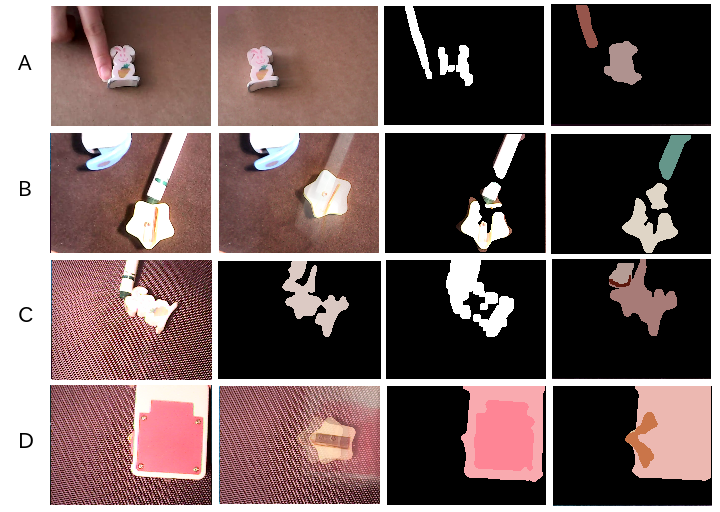
\includegraphics[width=0.75\textwidth]{7}
\label{figure:res}
\end{center}
\end{figure}

As discussed in Section \ref{sec:splitting}, background subtraction is causing degeneracy of extracted parts. We observed this phenomenon in our experiments. For example, in Figure \ref{figure:res} A, an object, that has been at rest, is moved by a finger to the right. The resulting extracted part for the finger is incomplete at the position where the object has been previously located. As the background average has more weight at where the object has been previously, background subtraction fails to detect the boundary of finger at that position. This happens regardless of the color of the finger and the object because the edges found by the Gabor filtering is usually colored white.

We also observed that image differencing can capture the movement of the entire finger (see Figure \ref{figure:res} A), suggesting a possibility that such degeneracy can be recovered using the motion image. 

A similar case is shown in Figure \ref{figure:res} B, where a star-shaped object is moved by a stick. The boundary of the object at the previous location is subtracted during the part extraction stage, resulting splitting in the inferred segment. Furthermore, the part within the boundary of the star-shaped object at the previous location appears to be wrongly matched as it contains more regions of the stick. This can be explained by the matching algorithm. The new part has no overlap with the inferred segment of the stick at the previous frame, resulting a negligible mutual information value with that segment. Indeed, the probability of taking the labelling of the stick is computed to be 2.6\%, while the probability for taking a new labelling, 97.4\%. Since that part also appears at the same time with the larger extracted part of the star-shaped object, the two parts are merged.

It may be possible that if the problematic part in the last example had overlap with the stick's inferred segment, our algorithm would be able to match them. This suggests that computing the mutual information of re-centered masked images may served to solve this problem. However, if two identical objects are in the scene, moving at different time, only using re-centered masked image may drive the algorithm match the second one that moves to the first one. A combination of the original construction with the re-centered mask image may work. 

In general, parts and segments merging and segment splitting appear to exhibit reasonable performance in our setting. We also observed that the recomputed labelling probabilities are often consistent before parts merging. This happens when our choice for the $D$ function often boost probabilities around to 90\% for matching that are consistent with the motion image, and probabilities around to 10\%, for those that are not.

The algorithm is the most delicate during part splitting. Figure \ref{figure:res} C shows an exampled of this case. The stick, previously segmented from the object, now touches the object and forms one extracted part. Our algorithm detected that the inferred object and stick segments match to that part. The transformation found by the optical flow shifts the inferred segments to match the current position of the objects. As show in the figure, no information about the position to split the part can be retrieved from the extracted part or from the motion image. 

The new segmentation produced by shifting the previously inferred segments is unfortunately often overlapping and covering background regions because the computed transformation may not correspond to the true motion of the objects. Furthermore, it destroys the method's ability to handle occluded objects. We observed that overlapping object often, if not always, form a part that need to be split. But the splitting algorithm assumes that all objects matched to that part move with the same motion. Thus occluded still object, transitioned from overlapping, will have their inferred segment shifted as if it has been moved. We can attempt to find the exact affine transformation for each segment by comparing whether each shifted segment lies within some proximity of the extracted part. Yet, the boundaries may largely differ, and the extra computational cost for obtaining the optical flow already drags the algorithm further away from real-time. 

Disabling part splitting, we test our method for occlusion. Figure \ref{figure:res} D shows an example of a object covering another. If the top object moves fast enough to cover the previously segmented bottom object, the inferred segment of the bottom object will have no match with the new parts and will stay without any update (except decaying). 

In summary, the inference and tracking can be done reliably using MI under some basic settings with simple objects. However, the method remains embarrassingly suboptimal due to incomplete object regions and the lack of optimal tuning. Part splitting also often slow down the process and alter the segments in the wrong way. Unfortunately, parts that need to be split occur often. Moreover, background subtraction tends to lose segments due to the shrinkage effect. We have attempted to reason on whether a matched previously inferred segment should not have its region updated, but it has only added more time complexity and badly handled edge cases. 

\section{Conclusion}

To respond to the need of unsupervised learning segmentation of objects in robotics, we developed a method that uses motion to produce segmentation of moved objects and a probabilistic matching algorithm to infer and track segments. Our foreground segmentation method using background subtraction and Gabor filtering lacks robustness to objects with complex shading or low contrast boundaries, and lacks generalizability to dark objects on bright background. Although our solution can exhibit some behaviour for handling certain optical effects such as overlapping and occlusion, due to the imperfections of part extraction algorithm and the lack of tuning, our implementation remains fragile and the solution often lose segments or occasionally explode into a plethora of segments even when there are only two objects in the scene. 

Perhaps our method can be combined with supervised methods. For example, combined with a FCN allows robots to learn and memorize objects found with the help of our method first in an uncluttered environment. Later, our method can be tuned to only extract novel object in a cluttered environment. In a large scaled image, we can employ tricks to optimize filtering and tracking, such as isolating moved regions for filtering and tracking only the objects in focus at a time. 

\begin{thebibliography}{9}

\bibitem{cogn1}
	A. N. Meltzoff
	\emph{Infant Imitation After a 1-Week Delay: Long-Term Memory for Novel Acts and Multiple Stimuli.}
	Developmental Psychology (1988) Vol 24, No 4, 470-476.
	
\bibitem{fcn}
	J. Long, E. Shelhamer, and T. Darrell. 
	\emph{Fully convolutionalnetworks for semantic segmentation.}
	CVPR, 2015

\bibitem{rnn}
	K. He, G. Gkioxari, P. Doll\`ar, R. Girshick
	\emph{Mask R-CNN.}
	
\bibitem{herke}
  H. V. Hoof, O. Kroemer, and J. Peters
  \emph{Probabilistic Segmentation and Targeted Exploration of Objects in Cluttered Environment.}
  
\bibitem{max-flow}
	P. Fitzpatrick and G. Metta 
	\emph{Grounding Vision Through Experimental Manipulation.}
	Philos. T. Roy. Soc. A (2003) Vol. 361, No. 1811, 2165-2185
	
\bibitem{kolmo}
	Y. Boykov and V. Kolmogorov
	\emph{An Experimental Comparison of Min-Cut/Max-Flow Algorithm for Energy Minimization in Vision.}
	Energy Minimization Methods in Computer Vision and Pattern Recognition (2001) 359-374

\bibitem{Gabor}
	D. C. Ciresan
	\emph{Flexible, High Performance Convolutional Neural Networks for Image Classification.}
	
\bibitem{tracking}
	A. Yilmaz
	\emph{Object Tracking: A Survey} ACM Computing Surveys, Vol. 38, No. 4, Article 13, Publication date: December 2006.

\bibitem{human-action}
	S. Park and J. K. Aggarwal
	\emph{Segmentation and Tracking of Interacting Human Body Parts Under Occlusion and Shadowing.} Workshop on Motion and Video Computing, Orlando, Florida (2002), 105-111

\bibitem{mi}
	J. P. W. Pluim
	\emph{Mutual Information based Registration of Medical Images: a Survey.}
	
\bibitem{rmi}
	D. B. Russakoff
	\emph{Image Similarity Using Mutual Information of Regions.}
	
\end{thebibliography}
%\end{multicols}
\end{document}